\documentclass[11pt]{article}

% ── Packages ──────────────────────────────────────────────────────────────────
\usepackage{amsmath, amsthm, amssymb}
\usepackage{geometry}
\usepackage{graphicx}
\usepackage{tikz}
\usetikzlibrary{angles}
\usepackage{hyperref}
\usepackage{enumitem}
\usepackage{xcolor}
\usepackage{mdframed}
\usepackage{float}
\geometry{margin=1in}
\hypersetup{colorlinks=true, linkcolor=blue!60!black, urlcolor=blue!60!black}

% ── Theorem Environments ──────────────────────────────────────────────────────
\theoremstyle{plain}
\newtheorem{theorem}{Theorem}[section]
\newtheorem{corollary}[theorem]{Corollary}
\newtheorem{lemma}[theorem]{Lemma}
\newtheorem{proposition}[theorem]{Proposition}

\theoremstyle{definition}
\newtheorem{definition}[theorem]{Definition}
\newtheorem{example}[theorem]{Example}
\newtheorem{remark}[theorem]{Remark}

% ── Macros ────────────────────────────────────────────────────────────────────
\newcommand{\Z}{\mathbb{Z}}
\newcommand{\R}{\mathbb{R}}
\newcommand{\Q}{\mathbb{Q}}
\newcommand{\N}{\mathbb{N}}
\newcommand{\vol}{\operatorname{vol}}
\newcommand{\conv}{\operatorname{conv}}
\newcommand{\cone}{\operatorname{cone}}

% ── Highlighted box for key ideas ─────────────────────────────────────────────
\newmdenv[
  backgroundcolor=blue!5,
  linecolor=blue!40,
  linewidth=1.2pt,
  roundcorner=4pt,
  skipabove=8pt,
  skipbelow=8pt
]{keybox}

% ── Title ─────────────────────────────────────────────────────────────────────
\begin{document}

\noindent
\begin{tabular}{|p{0.72\textwidth} r|}
\hline
\textbf{Recreational Mathematics Club} & \textit{Discussion \#2} \\[4pt]
\multicolumn{2}{|c|}{\Large All about lattices} \\[4pt]
Speakers: \textit{Mahek Shamsukha, Dhairya Baxi} & Indian Institute of Science \\
\hline
\end{tabular}


%% =============================================================================
\section{Lattices}
%% =============================================================================

Lattices are regular, discrete arrangements of points in Euclidean space. They arise naturally in crystallography, sphere packings, integer programming, cryptography, and coding theory. Two equivalent definitions are in common use.

\begin{definition}[Algebraic definition]
A \textbf{lattice} $\Lambda \subseteq \R^n$ is a \emph{discrete additive subgroup} of $\R^n$:
\begin{itemize}
  \item \textbf{Subgroup:} $\Lambda$ is closed under addition and subtraction.
  \item \textbf{Discrete:} There exists $\varepsilon > 0$ such that $\|x - y\| \ge \varepsilon$ for every pair of distinct points $x \ne y \in \Lambda$.
\end{itemize}
\end{definition}

\begin{definition}[Constructive / basis definition]
Let $B = [b_1, \ldots, b_k] \in \R^{n \times k}$ have linearly independent columns.
The \textbf{lattice generated by $B$} is
\[
  L(B) = \left\{\,\sum_{i=1}^{k} x_i\,b_i \;:\; x_i \in \Z\,\right\} = \{Bx : x \in \Z^k\}.
\]
The matrix $B$ is called a \textbf{basis}; $n$ and $k$ are the \textbf{dimension} and \textbf{rank}.
When $n = k$ the lattice is \textbf{full rank}.
\end{definition}

\begin{keybox}
\textbf{Key contrast with vector spaces.}
$\operatorname{span}(B) = \{Bx : x \in \R^k\}$ allows real coefficients and produces a continuous set.
$L(B) = \{Bx : x \in \Z^k\}$ restricts to integer coefficients, producing a \emph{discrete} set.
Since the columns $b_1,\ldots,b_k$ are linearly independent, any $y \in \operatorname{span}(B)$ has a unique representation $y = \sum x_i b_i$, and $y \in L(B)$ if and only if all $x_i \in \Z$.
\end{keybox}

\begin{example}
The standard integer lattice $\Z^n = \{(x_1,\dots,x_n) : x_i \in \Z\}$ is generated by the standard basis vectors of $\R^n$.
\end{example}

\begin{example}[$\Q^n$ is \emph{not} a lattice]
The set $\Q^n$ is a subgroup of $\R^n$ (it is closed under addition and subtraction), but it fails the discreteness condition. For any $\varepsilon > 0$, one can always find two distinct points $x, y \in \Q^n$ with $\|x - y\| < \varepsilon$ (e.g.\ take $x = 0$ and $y = (\varepsilon/2, 0, \ldots, 0)$), so no uniform lower bound on pairwise distances exists. Hence $\Q^n$ is \emph{not} a lattice.
\end{example}

%% =============================================================================
\section{Lattice Bases and Unimodular Transformations}
%% =============================================================================

A lattice can be represented by many different bases. Two bases $B$ and $C$ generate the same lattice if and only if $B = CU$ for some unimodular matrix $U$.

\begin{theorem}
$L(B) = L(C)$ if and only if there exists a \textbf{unimodular matrix} $U$ (a square integer matrix with $\det(U) = \pm 1$) such that $B = CU$.
\end{theorem}

\begin{proof}
$(\Leftarrow)$ Suppose $B = CU$ for some unimodular $U$. Since $\det(U) = \pm 1$ and $U$ has integer entries, $U^{-1}$ is also an integer matrix, and
\[
  C = BU^{-1}.
\]
Hence every column of $B$ is an integer combination of columns of $C$, giving $L(B) \subseteq L(C)$, and symmetrically $L(C) \subseteq L(B)$. Thus $L(B) = L(C)$.

\medskip
$(\Rightarrow)$ Suppose $L(B) = L(C)$. Since the columns of $B$ lie in $L(C)$, and vice versa, there exist integer matrices $V, W$ such that
\[
  B = CW \qquad \text{and} \qquad C = BV.
\]
Substituting the second into the first,
\[
  B = BVW \implies B(I - VW) = 0.
\]
Since the columns of $B$ are linearly independent, we conclude $VW = I$. Taking determinants on both sides,
\[
  \det(V) \cdot \det(W) = \det(I) = 1.
\]
Since $V, W$ have integer entries, $\det(V), \det(W) \in \Z$, so the only possibility is
\[
  \det(V) = \det(W) = \pm 1.
\]
Hence $W$ is unimodular, and $B = CW$ is the required relation with $U = W$. \qedhere
\end{proof}

%% =============================================================================
\section{Gram--Schmidt Orthogonalization}
%% =============================================================================

Given a lattice basis $B = [b_1, \ldots, b_n]$, it is often useful to transform it into an orthogonal system.

\begin{definition}
The \textbf{Gram--Schmidt orthogonalization} produces vectors $B^* = [b_1^*, \ldots, b_n^*]$ defined iteratively by
\[
  b_i^* = b_i - \sum_{j < i} \mu_{i,j}\,b_j^*, \qquad
  \mu_{i,j} = \frac{\langle b_i,\, b_j^*\rangle}{\langle b_j^*,\, b_j^*\rangle}.
\]
In matrix notation, $B = B^* M$ where $M$ is upper triangular with $1$s on the diagonal.
\end{definition}

The vectors $b_1^*, \ldots, b_n^*$ are mutually orthogonal and span the same vector space as $B$.
However, the orthogonal vectors are usually \textbf{not lattice vectors}.

\begin{example}
Consider the basis $B = \{b_1=(2,0),\, b_2=(1,2)\}$. The two diagrams below show
Gram--Schmidt applied in different orders. 

\bigskip
\begin{center}
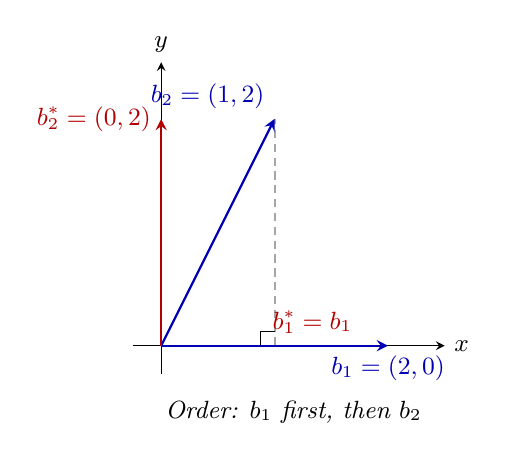
\begin{tikzpicture}[scale=1.2, >=stealth,
    bvec/.style={->, thick, blue!70!black},
    gsvec/.style={->, thick, red!70!black},
    proj/.style={densely dashed, gray!70, thick}]
  %--- Axes
  \draw[->] (-0.3,0) -- (3.0,0) node[right, font=\small] {$x$};
  \draw[->] (0,-0.3) -- (0,3.0) node[above, font=\small] {$y$};
  %--- Coordinates
  \coordinate (O)  at (0,0);
  \coordinate (B1) at (2.4,0);    % b1 = (2,0)
  \coordinate (B2) at (1.2,2.4);  % b2 = (1,2)
  \coordinate (F)  at (1.2,0);    % foot: projection of b2 onto b1
  %--- Projection lines
  \draw[proj] (O) -- (F);
  \draw[proj] (F) -- (B2);
  %--- Right angle at foot
  \draw (1.05,0) -- (1.05,0.15) -- (1.20,0.15);
  %--- Original vectors
  \draw[bvec] (O) -- (B1) node[below, font=\small] {$b_1=(2,0)$};
  \draw[bvec] (O) -- (B2) node[above left, font=\small] {$b_2=(1,2)$};
  %--- GS vectors (b1* = b1; b2* = (0,2))
  \draw[gsvec] (O) -- (0,2.4) node[left, font=\small] {$b_2^*=(0,2)$};
  \node[red!70!black, font=\small] at (1.6,0.25) {$b_1^*=b_1$};
  %--- Caption
  \node[font=\small\itshape] at (1.4,-0.7) {Order: $b_1$ first, then $b_2$};
\end{tikzpicture}
\hspace{1.5cm}
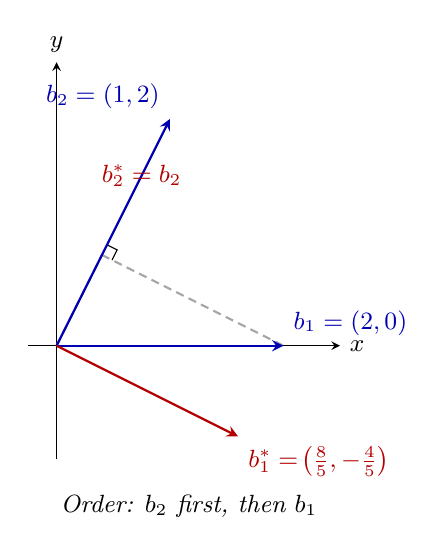
\begin{tikzpicture}[scale=1.2, >=stealth,
    bvec/.style={->, thick, blue!70!black},
    gsvec/.style={->, thick, red!70!black},
    proj/.style={densely dashed, gray!70, thick}]
  %--- Axes
  \draw[->] (-0.3,0) -- (3.0,0) node[right, font=\small] {$x$};
  \draw[->] (0,-1.2) -- (0,3.0) node[above, font=\small] {$y$};
  %--- Coordinates
  \coordinate (O)  at (0,0);
  \coordinate (B2) at (1.2,2.4);    % b2 = (1,2)
  \coordinate (B1) at (2.4,0);      % b1 = (2,0)
  \coordinate (F)  at (0.48,0.96);  % foot: projection of b1 onto b2
  \coordinate (BS1) at (1.92,-0.96);% b1* = (8/5, -4/5)
  %--- Projection lines
  \draw[proj] (O) -- (F);
  \draw[proj] (F) -- (B1);
  %--- Right angle at foot (between direction to B1 and direction to O)
  % Unit vec along b2* = (1,2)/sqrt(5); perp = (2,-1)/sqrt(5)
  \draw (0.5873,0.9064) -- (0.6410,1.0137) -- (0.5337,1.0673);
  %--- Original vectors
  \draw[bvec] (O) -- (B1) node[above right, font=\small] {$b_1=(2,0)$};
  \draw[bvec] (O) -- (B2) node[above left, font=\small] {$b_2=(1,2)$};
  %--- GS vectors (b2* = b2; b1* = (8/5, -4/5))
  \draw[gsvec] (O) -- (BS1) node[below right, font=\small] {$b_1^*=\!\left(\tfrac{8}{5},{-}\tfrac{4}{5}\right)$};
  \node[red!70!black, font=\small] at (0.9,1.8) {$b_2^*=b_2$};
  %--- Caption
  \node[font=\small\itshape] at (1.4,-1.7) {Order: $b_2$ first, then $b_1$};
\end{tikzpicture}
\end{center}
\end{example}

% \begin{remark}
% If $B$ is an integer matrix, then $\mu_{i,j} \in \Z / D_j$ where $D_j = \det(L(B_{j-1}))^2$.
% This shows the Gram--Schmidt procedure runs in polynomial time when $B$ is integer.
% \end{remark}

%% =============================================================================
\section{Fundamental Parallelepiped and Determinant}
%% =============================================================================

Given a lattice basis $B = [b_1, \ldots, b_n]$, we define the \textbf{fundamental parallelepiped}
\[
  \mathcal{P}(B) = \Bigl\{\,\sum_{i=1}^{n} x_i\,b_i : 0 \le x_i < 1\,\Bigr\}.
\]
The translates $\mathcal{P}(B) + v$ for $v \in L(B)$ partition all of $\R^n$; each coset of the lattice has exactly one representative in $\mathcal{P}(B)$.

\begin{definition}
The \textbf{determinant} of a lattice is the volume of the fundamental parallelepiped:
\[
  \det(L(B)) = \vol(\mathcal{P}(B)) = \prod_{i=1}^{n} \|b_i^*\|.
\]
\end{definition}

Geometrically, $\det(L)$ measures the \textbf{inverse density} of lattice points: a large region of volume $V$ contains roughly $V/\det(L)$ lattice points. The determinant does not depend on the choice of basis.

\begin{proposition}
For any lattice basis $B$,
\[
  \det(L(B)) = \sqrt{\det(B^\top B)}.
\]
In particular, if $B \in \R^{n \times n}$ is square, then $\det(L(B)) = |\det(B)|$.
\end{proposition}

\begin{proof}
From the Gram--Schmidt factorisation $B = B^* M$, where $M$ is upper triangular with $1$s on the diagonal, we compute
\[
  \det(B^\top B) = \det(M^\top {B^*}^\top B^* M) = \det(M^\top)\,\det({B^*}^\top B^*)\,\det(M).
\]
Since $M$ is upper triangular with $1$s on the diagonal, $\det(M) = \det(M^\top) = 1$. Since the columns of $B^*$ are orthogonal, ${B^*}^\top B^*$ is diagonal with entries $\|b_i^*\|^2$, so
\[
  \det({B^*}^\top B^*) = \prod_{i} \|b_i^*\|^2 = \det(L(B))^2.
\]
Taking the square root,
\[
  \sqrt{\det(B^\top B)} = \det(L(B)). \qedhere
\]
\end{proof}

\begin{theorem}
Let $B \in \Z^{n \times n}$ be nonsingular and let $d = |\det(B)|$. Then $d\,\Z^n \subseteq L(B)$.
\end{theorem}

\begin{proof}
Let $v \in d\,\Z^n$ be arbitrary, so $v = d\,y$ for some $y \in \Z^n$. We wish to find $x \in \Z^n$ such that
\[
  Bx = v = d\,y.
\]
Recall the \textbf{adjugate} (classical adjoint) $\operatorname{adj}(B)$, whose $(i,j)$ entry is the signed $(j,i)$ cofactor of $B$. Since $B \in \Z^{n\times n}$, every cofactor is an integer determinant, so
\[
  \operatorname{adj}(B) \in \Z^{n \times n}.
\]
The key identity relating the adjugate to the inverse is
\[
  B \cdot \operatorname{adj}(B) = \det(B)\, I = d\, I.
\]
Set $x = \operatorname{adj}(B)\,y$. Since $\operatorname{adj}(B)$ and $y$ are both integer, $x \in \Z^n$. Moreover,
\[
  Bx = B\,\operatorname{adj}(B)\,y = d\,I\,y = d\,y = v.
\]
Hence $v = Bx \in L(B)$, and since $v$ was arbitrary, $d\,\Z^n \subseteq L(B)$.
\end{proof}

This shows that every integer lattice contains a scaled copy of the standard lattice as a sublattice.

%% =============================================================================
\section{Minimum Distance and Shortest Vectors}
%% =============================================================================

\begin{definition}
The \textbf{minimum distance} of a lattice $\Lambda$ is
\[
  \lambda_1(\Lambda) = \min_{x \in \Lambda \setminus \{0\}} \|x\|.
\]
\end{definition}

This corresponds to the length of the shortest nonzero lattice vector. More generally, the \textbf{successive minima} $\lambda_1 \le \lambda_2 \le \cdots \le \lambda_n$ are defined so that $\lambda_k(\Lambda)$ is the smallest $r$ such that $\Lambda$ contains $k$ linearly independent vectors of length at most $r$.

\begin{theorem}
For a lattice basis $B$ with Gram--Schmidt vectors $b_i^*$,
\[
  \lambda_1(L(B)) \;\ge\; \min_i \|b_i^*\|.
\]
\end{theorem}

%% =============================================================================
\section{Blichfeldt's Theorem}
%% =============================================================================

Blichfeldt's theorem is essentially the \textbf{pigeonhole principle for volumes}: if a set $S$ is too large to fit inside a single fundamental parallelepiped, then when we tile space with translates of $\mathcal{P}(B)$, at least two pieces of $S$ must land in the same cell — and shifting them back reveals two points of $S$ that differ by a lattice vector.

\begin{theorem}[Blichfeldt]
Let $\Lambda = L(B)$ be a lattice and $S \subset \R^n$ a measurable set. If $\vol(S) > \det(\Lambda)$,
then there exist two distinct points $z_1, z_2 \in S$ such that $z_1 - z_2 \in \Lambda$.
\end{theorem}

\begin{proof}
Decompose $S$ into the pieces that lie in each lattice-translate of $\mathcal{P}(B)$:
\[
  S_x \;=\; S \cap \bigl(x + \mathcal{P}(B)\bigr), \qquad x \in \Lambda.
\]
These sets are pairwise disjoint and cover $S$, so
\[
  \vol(S) \;=\; \sum_{x \in \Lambda} \vol(S_x).
\]
Now translate each piece back into $\mathcal{P}(B)$ by defining $T_x = S_x - x \subseteq \mathcal{P}(B)$. Since translation preserves volume,
\[
  \sum_{x \in \Lambda} \vol(T_x) \;=\; \sum_{x \in \Lambda} \vol(S_x) \;=\; \vol(S) \;>\; \det(\Lambda) \;=\; \vol(\mathcal{P}(B)).
\]
Since all $T_x$ live inside $\mathcal{P}(B)$ and their total volume exceeds $\vol(\mathcal{P}(B))$, they cannot all be disjoint. Hence there exist distinct $x \neq y \in \Lambda$ such that $T_x \cap T_y \neq \emptyset$. Pick any point $p$ in this intersection. Then
\[
  z_1 = p + x \in S_x \subseteq S, \qquad z_2 = p + y \in S_y \subseteq S,
\]
and
\[
  z_1 - z_2 \;=\; x - y \;\in\; \Lambda. \qedhere
\]
\end{proof}

\noindent The diagram below illustrates the idea in $\R^2$: a blob $S$ is cut by the lattice tiling, each piece is translated into $\mathcal{P}(B)$, and two pieces overlap.

\begin{center}
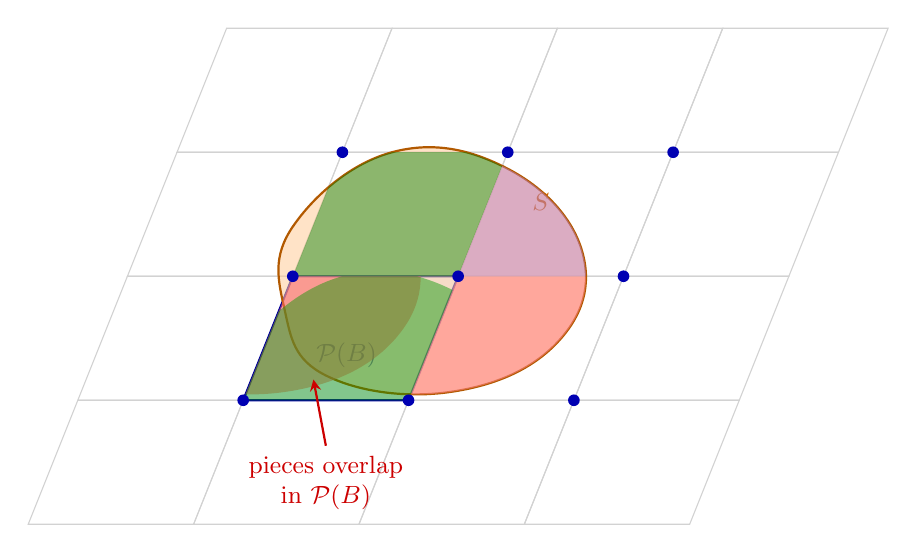
\begin{tikzpicture}[scale=1.05, >=stealth]

  % ── grid of parallelepipeds ──────────────────────────────────────────────
  % basis b1=(2,0), b2=(0.6,1.5)
  \def\ax{2.0}\def\ay{0.0}
  \def\bx{0.6}\def\by{1.5}

  \foreach \i in {-1,0,1,2}{
    \foreach \j in {-1,0,1,2}{
      \draw[gray!35, thin]
        ({\i*\ax+\j*\bx},    {\i*\ay+\j*\by}) --
        ({\i*\ax+\j*\bx+\ax},{\i*\ay+\j*\by+\ay}) --
        ({\i*\ax+\j*\bx+\ax+\bx},{\i*\ay+\j*\by+\ay+\by}) --
        ({\i*\ax+\j*\bx+\bx},{\i*\ay+\j*\by+\by}) -- cycle;
    }
  }

  % ── highlight the fundamental cell ──────────────────────────────────────
  \fill[blue!10, opacity=0.7]
    (0,0) -- (\ax,\ay) -- (\ax+\bx,\ay+\by) -- (\bx,\by) -- cycle;
  \draw[blue!60!black, thick]
    (0,0) -- (\ax,\ay) -- (\ax+\bx,\ay+\by) -- (\bx,\by) -- cycle;
  \node[blue!60!black, font=\small] at (1.25,0.55) {$\mathcal{P}(B)$};

  % ── blob S ───────────────────────────────────────────────────────────────
  \begin{scope}
    \clip (-0.5,-0.4) rectangle (5.5,3.5);
    \fill[orange!40, opacity=0.55]
      plot[smooth cycle, tension=0.7] coordinates
        {(1.0,0.3)(2.5,0.1)(3.8,0.7)(4.1,1.8)(3.2,2.8)(1.8,3.0)(0.6,2.1)(0.5,1.1)};
    \draw[orange!70!black, thick]
      plot[smooth cycle, tension=0.7] coordinates
        {(1.0,0.3)(2.5,0.1)(3.8,0.7)(4.1,1.8)(3.2,2.8)(1.8,3.0)(0.6,2.1)(0.5,1.1)};
  \end{scope}
  \node[orange!80!black, font=\small\itshape] at (3.6,2.4) {$S$};

  % ── coloured pieces of S inside neighbouring cells ───────────────────────
  % piece in cell (1,0): clip to that cell
  \begin{scope}
    \clip ({\ax},{\ay}) -- ({2*\ax},{2*\ay}) -- ({2*\ax+\bx},{2*\ay+\by}) -- ({\ax+\bx},{\ay+\by}) -- cycle;
    \fill[red!50, opacity=0.6]
      plot[smooth cycle, tension=0.7] coordinates
        {(1.0,0.3)(2.5,0.1)(3.8,0.7)(4.1,1.8)(3.2,2.8)(1.8,3.0)(0.6,2.1)(0.5,1.1)};
  \end{scope}

  % piece in cell (0,1)
  \begin{scope}
    \clip ({\bx},{\by}) -- ({\ax+\bx},{\ay+\by}) -- ({\ax+2*\bx},{\ay+2*\by}) -- ({2*\bx},{2*\by}) -- cycle;
    \fill[green!50!black, opacity=0.45]
      plot[smooth cycle, tension=0.7] coordinates
        {(1.0,0.3)(2.5,0.1)(3.8,0.7)(4.1,1.8)(3.2,2.8)(1.8,3.0)(0.6,2.1)(0.5,1.1)};
  \end{scope}

  % piece in cell (1,1)
  \begin{scope}
    \clip ({\ax+\bx},{\ay+\by}) -- ({2*\ax+\bx},{2*\ay+\by}) -- ({2*\ax+2*\bx},{2*\ay+2*\by}) -- ({\ax+2*\bx},{\ay+2*\by}) -- cycle;
    \fill[violet!50, opacity=0.55]
      plot[smooth cycle, tension=0.7] coordinates
        {(1.0,0.3)(2.5,0.1)(3.8,0.7)(4.1,1.8)(3.2,2.8)(1.8,3.0)(0.6,2.1)(0.5,1.1)};
  \end{scope}

  % ── translated pieces into P(B), with overlap shown ───────────────────────
  % red piece translated by -b1 = -(2,0)
  \begin{scope}[xshift=-\ax cm, yshift=-\ay cm]
    \begin{scope}
      \clip ({\ax},{\ay}) -- ({2*\ax},{2*\ay}) -- ({2*\ax+\bx},{2*\ay+\by}) -- ({\ax+\bx},{\ay+\by}) -- cycle;
      \fill[red!60, opacity=0.55, xshift=0cm]
        plot[smooth cycle, tension=0.7] coordinates
          {(1.0,0.3)(2.5,0.1)(3.8,0.7)(4.1,1.8)(3.2,2.8)(1.8,3.0)(0.6,2.1)(0.5,1.1)};
    \end{scope}
  \end{scope}

  % green piece translated by -b2 = -(0.6,1.5)
  \begin{scope}[xshift=-\bx cm, yshift=-\by cm]
    \begin{scope}
      \clip ({\bx},{\by}) -- ({\ax+\bx},{\ay+\by}) -- ({\ax+2*\bx},{\ay+2*\by}) -- ({2*\bx},{2*\by}) -- cycle;
      \fill[green!60!black, opacity=0.45]
        plot[smooth cycle, tension=0.7] coordinates
          {(1.0,0.3)(2.5,0.1)(3.8,0.7)(4.1,1.8)(3.2,2.8)(1.8,3.0)(0.6,2.1)(0.5,1.1)};
    \end{scope}
  \end{scope}

  % ── lattice points ────────────────────────────────────────────────────────
  \foreach \i in {0,1,2}{
    \foreach \j in {0,1,2}{
      \fill[blue!70!black] ({\i*\ax+\j*\bx},{\i*\ay+\j*\by}) circle (2pt);
    }
  }

  % ── overlap annotation ────────────────────────────────────────────────────
  \draw[->, thick, red!80!black]
    (1.0, -0.55) node[below, font=\small, align=center]
      {pieces overlap\\in $\mathcal{P}(B)$} -- (0.85, 0.25);

\end{tikzpicture}
\end{center}

%% =============================================================================
\section{Minkowski's Convex Body Theorem}
%% =============================================================================

\begin{theorem}[Minkowski]
Let $\Lambda$ be a lattice in $\R^n$ and let $S$ be a convex, centrally symmetric body. If
\[
  \vol(S) > 2^n \det(\Lambda),
\]
then $S$ contains a nonzero lattice point.
\end{theorem}

\begin{proof}
Apply Blichfeldt to $S/2 = \{x : 2x \in S\}$, which satisfies $\vol(S/2) = 2^{-n}\vol(S) > \det(\Lambda)$.
Blichfeldt gives distinct $z_1, z_2 \in S/2$ with $z_1 - z_2 \in \Lambda \setminus \{0\}$.
Then $2z_1, 2z_2 \in S$, so by symmetry $-2z_2 \in S$, and by convexity
\[
  z_1 - z_2 = \tfrac{1}{2}(2z_1) + \tfrac{1}{2}(-2z_2) \;\in\; S. \qedhere
\]
\end{proof}

This theorem gives an upper bound on the shortest lattice vector:
\[
  \lambda_1(\Lambda) \;\le\; \sqrt{n}\,\det(\Lambda)^{1/n}.
\]

%% =============================================================================
\section{Application: Primes of the Form $a^2 + b^2$}
%% =============================================================================

\begin{theorem}
If $p$ is a prime with $p \equiv 1 \pmod{4}$, then $p = a^2 + b^2$ for some integers $a, b$.
\end{theorem}

\begin{proof}[Idea of the proof]
Since $p \equiv 1 \pmod{4}$, there exists $i$ such that $i^2 \equiv -1 \pmod{p}$.

Consider the lattice generated by
\[
  B = \begin{pmatrix} 1 & 0 \\ i & p \end{pmatrix}.
\]
By Minkowski's theorem, there exists a nonzero lattice vector $(a,b)^\top$ satisfying $0 < a^2 + b^2 < 2p$.
Using $i^2 \equiv -1 \pmod{p}$, one checks that $p \mid a^2 + b^2$. Since the value lies strictly between $0$ and $2p$, we must have $a^2 + b^2 = p$.
\end{proof}

%% =============================================================================
\section{Hermite Normal Form}
%% =============================================================================

The Hermite Normal Form (HNF) provides a canonical, unique representation for a lattice. We say a matrix $B = [b_1,\ldots,b_n]$ of full row rank is in HNF if it has the form $B = [H \mid 0]$, where:

\begin{definition}
A square matrix $H = [h_{ij}]$ is in \textbf{Hermite Normal Form} if:
\begin{itemize}
  \item $h_{ij} = 0$ for $i < j$ \quad (i.e., $H$ is lower triangular), and
  \item $0 \le h_{ij} < h_{ii}$ for $i > j$ \quad (i.e., off-diagonal entries are non-negative and strictly less than the diagonal entry on the same row).
\end{itemize}
\end{definition}

In particular, $H$ is nonsingular. The HNF is computed by applying elementary column operations, which are special unimodular transformations:
\begin{enumerate}
  \item Swap two columns: $b_i \leftrightarrow b_j$.
  \item Multiply a column by $-1$: $b_i \leftarrow -b_i$.
  \item Add an integer multiple of one column to another: $b_i \leftarrow b_i + \alpha b_j$, $\alpha \in \Z$.
\end{enumerate}
Since these are unimodular, they preserve the lattice generated by the columns of $B$.

\begin{theorem}[Existence of HNF]
Every rational matrix of full row rank can be brought into Hermite normal form by a sequence of elementary column operations. Equivalently, for every such matrix $B$ there is a unimodular matrix $U$ such that $BU$ is in HNF.
\end{theorem}

\begin{proof}
Without loss of generality assume $B$ is integral (otherwise clear denominators). We build a sequence of matrices
\[
  B_k = \begin{pmatrix} H_k & 0 \\ C_k & D_k \end{pmatrix},
\]
where $H_k$ is a $k\times k$ matrix already in HNF. At each step, let $d_1,\ldots,d_{n-k}$ be the first-row entries of $D_k$. By permuting columns and negating, assume all $d_i \ge 0$ with at least one nonzero. If two nonzero entries $d_i > d_j$ appear, add $-\lfloor d_i/d_j \rfloor$ times column $j$ to column $i$, strictly reducing the total sum of first-row entries. Repeating (this executes the Euclidean algorithm on pairs of entries) terminates with a single nonzero entry $d$ in the first row of $D_k$, which is placed in the first column by a swap. Finally, for each $i = 1,\ldots,k$, subtract $\lfloor c_i/d \rfloor$ times the new column from column $i$ to reduce all entries in the first row of $C_k$ to the range $[0, d)$. This yields $B_{k+1}$ with $H_{k+1}$ of size $(k+1)\times(k+1)$ in HNF.
\end{proof}

\begin{remark}
The naive algorithm above may be non-polynomial due to intermediate entry growth. A polynomial-time variant exists by performing all arithmetic modulo the determinant of the relevant submatrix, keeping entries bounded throughout.
\end{remark}

\subsection*{Sublattices and the Index}

Let $\Lambda' = L(B')$ be a sublattice of $\Lambda = L(B)$, both full-dimensional. Then $B' = BV$ for some integral matrix $V$, and the \textbf{index} of $\Lambda'$ in $\Lambda$ is
\[
  D(\Lambda, \Lambda') \;:=\; |\det(V)| \;=\; \frac{\det(\Lambda')}{\det(\Lambda)} \;\in\; \Z_{>0}.
\]

\begin{lemma}
If $\Lambda'$ is a sublattice of $\Lambda$ with index $D$, then
\[
  D\Lambda \;\subseteq\; \Lambda' \;\subseteq\; \Lambda.
\]
\end{lemma}

\begin{proof}
Let $B, B'$ be bases of $\Lambda, \Lambda'$ with $B' = BV$ and $D = |\det(V)|$. Then $B = B' V^{-1}$ and $DV^{-1}$ is an integral matrix (since the entries of $V^{-1} = \operatorname{adj}(V)/\det(V)$ become integral upon multiplication by $D$). Hence
\[
  DB = B'(DV^{-1}) \;\in\; L(B') = \Lambda',
\]
so $D\Lambda \subseteq \Lambda'$.
\end{proof}

\begin{theorem}[Bases in HNF]
Let $\Lambda'$ be a sublattice of $\Lambda$.
\begin{enumerate}[label=(\alph*)]
  \item For every basis $B$ of $\Lambda$, there is a unique basis $B'$ of $\Lambda'$ such that $B' = BH$ with $H$ in HNF.
  \item For every basis $B'$ of $\Lambda'$, there is a unique basis $B$ of $\Lambda$ such that $B' = BH$ with $H$ in HNF.
\end{enumerate}
\end{theorem}

%% =============================================================================
\section{Easy and Hard Lattice Problems}
%% =============================================================================

Using HNF and the dual lattice, the following problems are all solvable in polynomial time: computing a basis for $L(B)$, deciding whether $L(B) = L(C)$, membership testing ($v \in L(B)$?), union, and containment.

In contrast, the following are believed to be computationally hard.

\begin{definition}
The \textbf{Shortest Vector Problem (SVP)}: given a lattice basis $B$, find a nonzero lattice vector of length at most $\gamma \cdot \lambda_1(L(B))$.
\end{definition}

\begin{definition}
The \textbf{Shortest Independent Vectors Problem (SIVP)}: given a rank-$n$ basis $B$, find $n$ linearly independent lattice vectors of length at most $\gamma \cdot \lambda_n(L(B))$.
\end{definition}

\begin{definition}
The \textbf{Closest Vector Problem (CVP)}: given a basis $B$ and a target vector $t$, find a lattice vector within distance $\gamma \cdot \operatorname{dist}(t, L(B))$.
\end{definition}

% ══════════════════════════════════════════════════════════════════════════════
\section*{Acknowledgements}
% ══════════════════════════════════════════════════════════════════════════════

These notes follow the exposition in:
\begin{itemize}
  \item D.~Micciancio, \textit{CSE 206A: Lattice Algorithms and Applications}, 
        Winter 2010, UC San Diego.
  \item HNF section from the lecture notes on lattices, available at 
        \url{https://www.epfl.ch/labs/disopt/wp-content/uploads/2018/09/lattices.pdf}.
\end{itemize}
\end{document}